%\documentclass[journal]{vgtc}                % final (journal style)
\documentclass[review,journal]{vgtc}         % review (journal style)
%\documentclass[widereview]{vgtc}             % wide-spaced review
%\documentclass[preprint,journal]{vgtc}       % preprint (journal style)
%\documentclass[electronic,journal]{vgtc}     % electronic version, journal

%% Uncomment one of the lines above depending on where your paper is
%% in the conference process. ``review'' and ``widereview'' are for review
%% submission, ``preprint'' is for pre-publication, and the final version
%% doesn't use a specific qualifier. Further, ``electronic'' includes
%% hyperreferences for more convenient online viewing.

%% Please use one of the ``review'' options in combination with the
%% assigned online id (see below) ONLY if your paper uses a double blind
%% review process. Some conferences, like IEEE Vis and InfoVis, have NOT
%% in the past.

%% Please note that the use of figures other than the optional teaser is not permitted on the first page
%% of the journal version.  Figures should begin on the second page and be
%% in CMYK or Grey scale format, otherwise, colour shifting may occur
%% during the printing process.  Papers submitted with figures other than the optional teaser on the
%% first page will be refused.

%% These three lines bring in essential packages: ``mathptmx'' for Type 1
%% typefaces, ``graphicx'' for inclusion of EPS figures. and ``times''
%% for proper handling of the times font family.

\usepackage{mathptmx}
\usepackage{graphicx}
\usepackage{times}
\usepackage{enumerate}
\usepackage{color}
\usepackage{bm}
\usepackage{amsmath}
\usepackage{subfigure}

%% We encourage the use of mathptmx for consistent usage of times font
%% throughout the proceedings. However, if you encounter conflicts
%% with other math-related packages, you may want to disable it.

%% This turns references into clickable hyperlinks.
\usepackage[bookmarks,backref=true,linkcolor=black]{hyperref} %,colorlinks
\hypersetup{
  pdfauthor = {},
  pdftitle = {},
  pdfsubject = {},
  pdfkeywords = {},
  colorlinks=true,
  linkcolor= black,
  citecolor= black,
  pageanchor=true,
  urlcolor = black,
  plainpages = false,
  linktocpage
}
\tolerance=1
\emergencystretch=\maxdimen
\hyphenpenalty=10000
\hbadness=10000
%% If you are submitting a paper to a conference for review with a double
%% blind reviewing process, please replace the value ``0'' below with your
%% OnlineID. Otherwise, you may safely leave it at ``0''.
\onlineid{234}
\newcommand{\note}[1]{\iffalse #1 \fi}
\newcommand{\col}[1]{{\color{blue}{#1}}}

%% declare the category of your paper, only shown in review mode
\vgtccategory{Research}

%% allow for this line if you want the electronic option to work properly
\vgtcinsertpkg

%% In preprint mode you may define your own headline.
%\preprinttext{To appear in an IEEE VGTC sponsored conference.}

%% Paper title.

\title{Exploring High Dimensional Data Through\\ Locally Optimized Projections}

%% This is how authors are specified in the journal style

%% indicate IEEE Member or Student Member in form indicated below
%%\author{Roy G. Biv, Ed Grimley, \textit{Member, IEEE}, and Martha Stewart}
%%\authorfooter{
%% insert punctuation at end of each item
%%\item
 %%Roy G. Biv is with Starbucks Research. E-mail: roy.g.biv@aol.com.
%%\item
%% Ed Grimley is with Grimley Widgets, Inc.. E-mail: ed.grimley@aol.com.
%%\item
%% Martha Stewart is with Martha Stewart Enterprises at Microsoft
%% Research. E-mail: martha.stewart@marthastewart.com.
%%}

%other entries to be set up for journal
%% \shortauthortitle{Biv \MakeLowercase{\textit{et al.}}: Global Illumination for Fun and Profit}
%\shortauthortitle{Firstauthor \MakeLowercase{\textit{et al.}}: Paper Title}

%% Abstract section.
\abstract{Dimension reduced projection is usually obtained via a global optimization. It gives a good overview of the data, but is not suitable for local data analysis. That's because any local relationship in the projection could be unfaithful due to projection distortions. To address this problem, we propose an interactive exploration method, to help users customize linear projections for a better local analysis. Specifically, we allow users to define their point of interest (POI) data. Then regarding different analytic purposes, we generate multiple projections to enhance different features of the POI. We also reveal relationships among different POIs, by comparing their featured projections. At last, our method is proved effective via case studies with real-world datasets.
} % end of abstract

%% Keywords that describe your work. Will show as 'Index Terms' in journal
%% please capitalize first letter and insert punctuation after last keyword
\keywords{Dimension-reduced projection, local analysis, high-dimensional data}

%% ACM Computing Classification System (CCS).
%% See <http://www.acm.org/class/1998/> for details.
%% The ``\CCScat'' command takes four arguments.

\CCScatlist{ % not used in journal version
 \CCScat{K.6.1}{Management of Computing and Information Systems}%
{Project and People Management}{Life Cycle};
 \CCScat{K.7.m}{The Computing Profession}{Miscellaneous}{Ethics}
}

%% Uncomment below to include a teaser figure.
  \teaser{
 \centering
 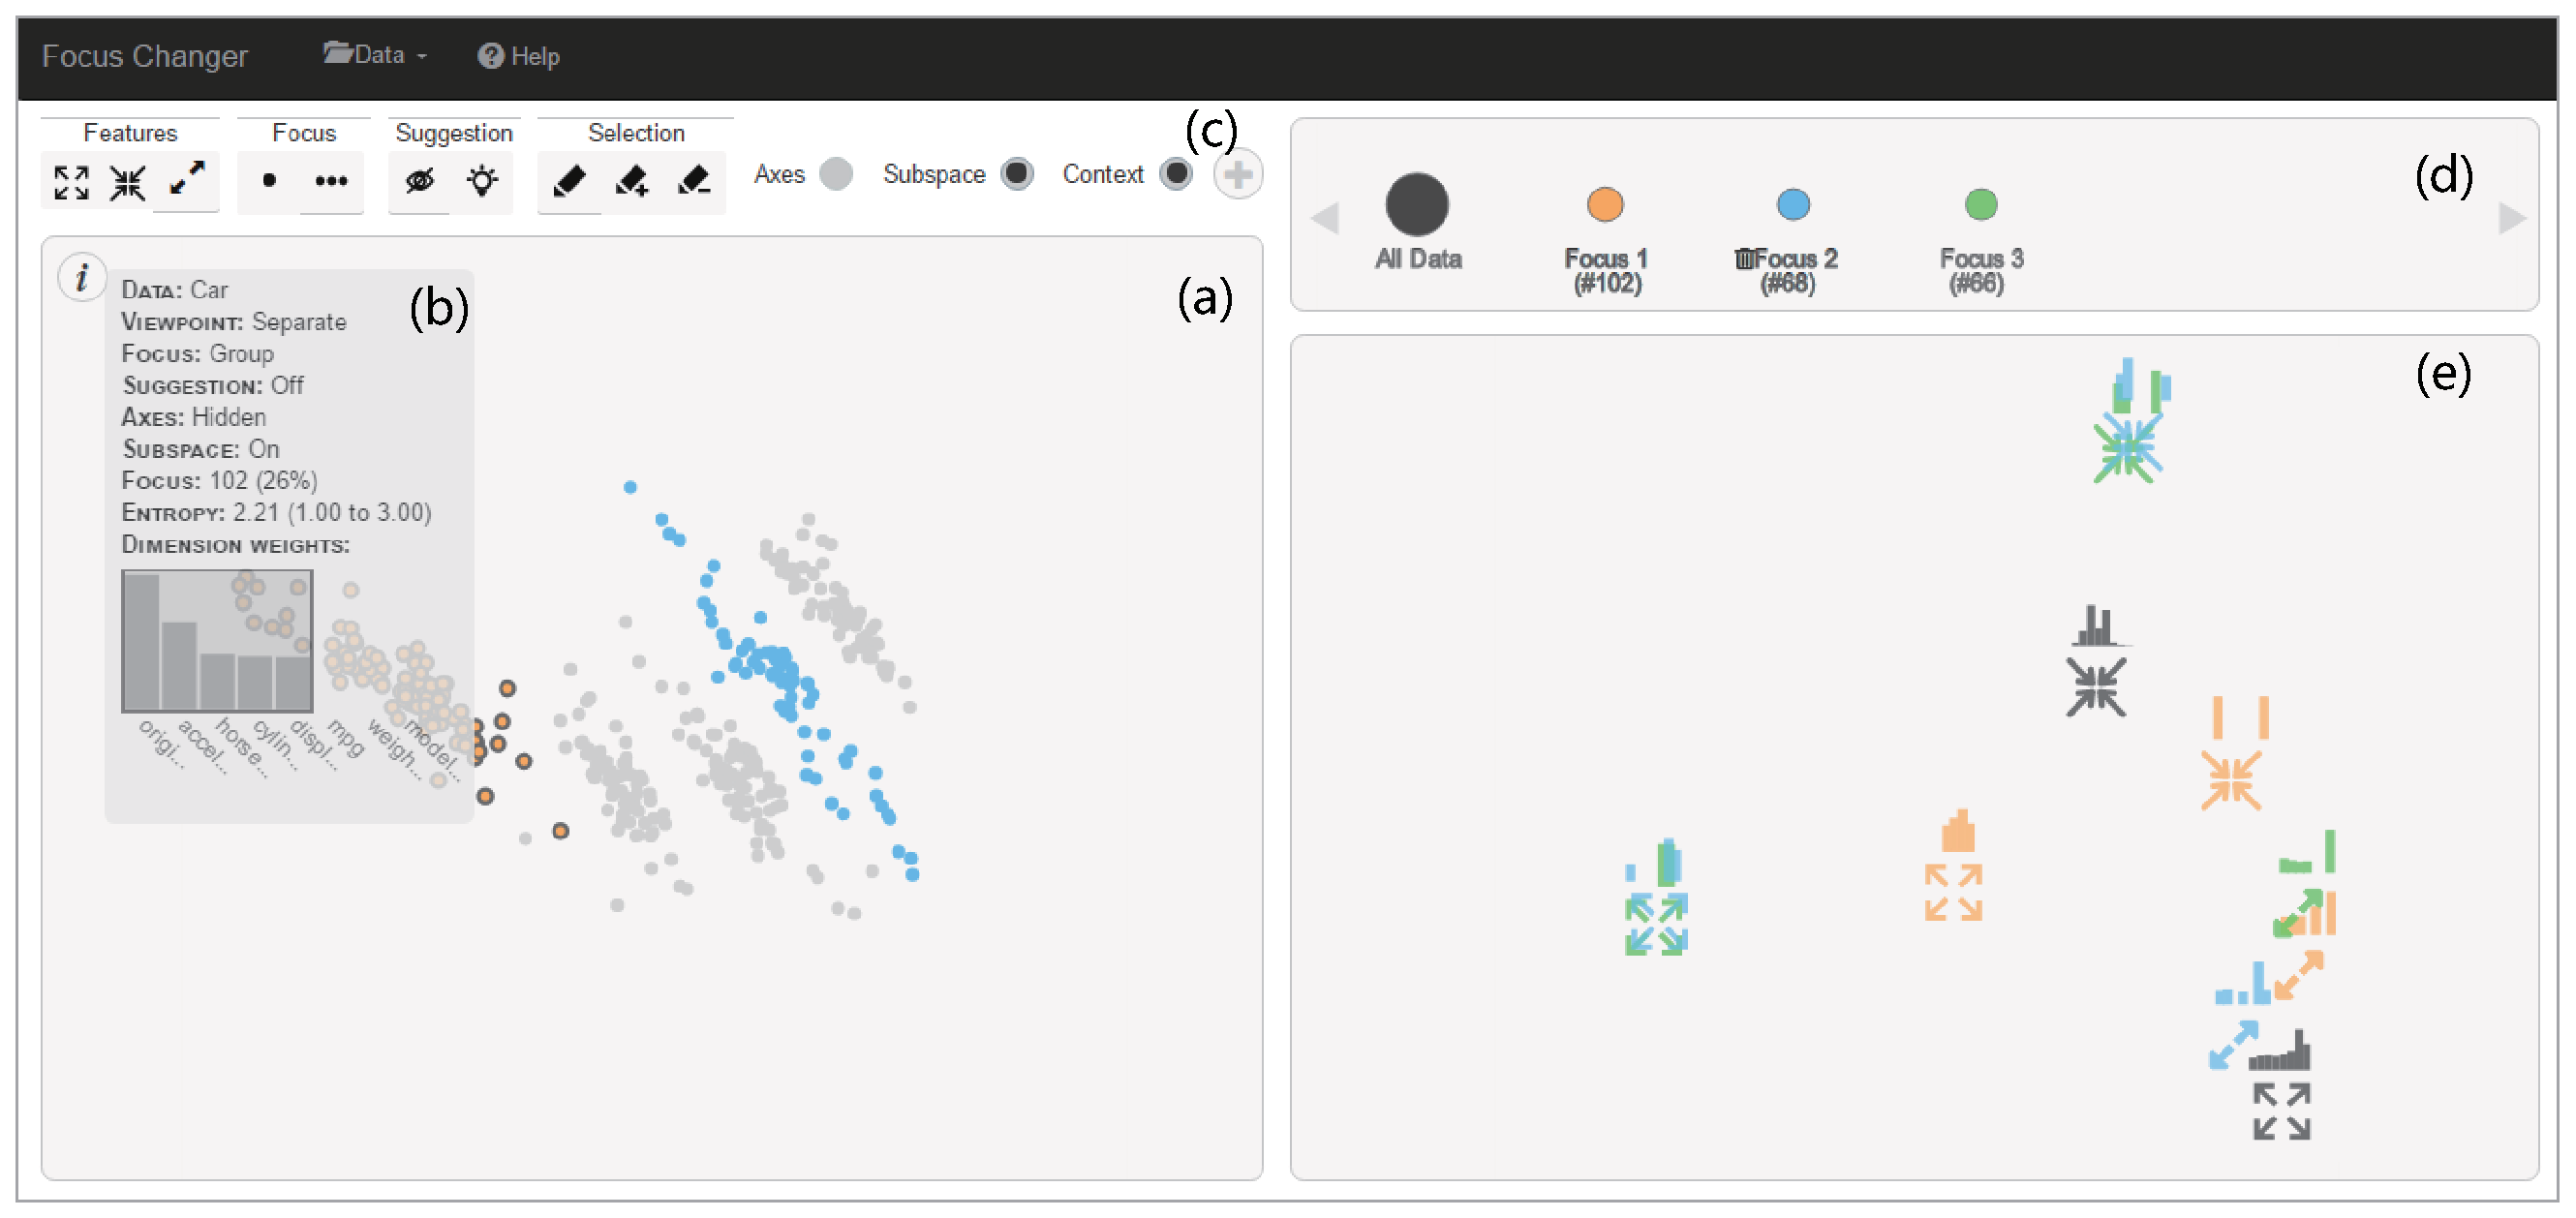
\includegraphics[width=1\linewidth]{images/teaser.eps}
  \caption{Teaser here.}
  }

%% Uncomment below to disable the manuscript note
%\renewcommand{\manuscriptnotetxt}{}

%% Copyright space is enabled by default as required by guidelines.
%% It is disabled by the 'review' option or via the following command:
% \nocopyrightspace

%%%%%%%%%%%%%%%%%%%%%%%%%%%%%%%%%%%%%%%%%%%%%%%%%%%%%%%%%%%%%%%%
%%%%%%%%%%%%%%%%%%%%%% START OF THE PAPER %%%%%%%%%%%%%%%%%%%%%%
%%%%%%%%%%%%%%%%%%%%%%%%%%%%%%%%%%%%%%%%%%%%%%%%%%%%%%%%%%%%%%%%%

\begin{document}

%% The ``\maketitle'' command must be the first command after the
%% ``\begin{document}'' command. It prepares and prints the title block.

%% the only exception to this rule is the \firstsection command

%% \section{Introduction} %for journal use above \firstsection{..} instead
\firstsection{Introduction}
\maketitle
Dimension-reduced projection is widely used for high-dimensional data analysis. It seeks to approximate the original distribution in a low-dimensional space. Such approximation is often globally optimized to make a good overview of the data. But due to approximation errors, data relationships will inevitably be distorted. The distortions are hard to ignore when it comes to local data. They largely harm the perception of local structures, yet are often transparent to users. Even if distortions are shown in the projection~\cite{DBLP:journals/tvcg/StahnkeDMT16}~\cite{DBLP:journals/ijon/Aupetit07}, users have no means to control their distribution. In general, globally optimized projections make good overviews, but are not suitable for local data analysis.
%change citation here.

One way to alleviate this problem, is to observe the data in a different perspective. Some previous works~\cite{DBLP:journals/cgf/JeongZFRC09}~\cite{DBLP:journals/tvcg/NamM13}~\cite{DBLP:journals/tvcg/LehmannT13} allow users to change the projection by adjusting dimension weights. It helps to clarify detailed structures and find out more useful information. To help build a targeted analysis, featured clusters are often provided beforehand~\cite{DBLP:journals/tvcg/NamM13}~\cite{DBLP:journals/cgf/LiuWTBP15}. However, users know nothing about the given clusters. They have to solve their puzzles by manually searching the enormous data space. It's a blinded and exhausting process, where users have no clue how to steer the dimensions to get a better view. Even if interesting projections are found, it's hard to explain or assess them without distortion information.

Compared to dimension-based exploration, feature-based mining techniques are more efficient in revealing informative projections. Projection pursuit~\cite{DBLP:journals/tc/FriedmanT74} searches for projections to optimize predefined indices. The rank-by-feature framework~\cite{DBLP:journals/ivs/SeoS05} ranks a series of projections by their interestingness. In more recent works, users are involved to specify desired features~\cite{DBLP:journals/tvcg/JohanssonJ09} and relationships~\cite{DBLP:journals/tvcg/HuBMHNL13}~\cite{DBLP:journals/tvcg/Gleicher13}. These methods, though effective, largely depend on predefined metrics or users' prior knowledge. It makes them unsuitable for an interactive exploration starting from scratch. Besides, little attention had been paid to facilitate local data analysis.

In this work, we propose an interactive exploration method, that promotes consecutive local data analyses in locally optimized projections.

\note{
Nevertheless, local analysis is not only necessary, but also an efficient way to explore high-dimensional data. On one hand, a sole overview cannot show all aspects.\note{especially when the dimensionality is high.} After a quick glance, users tend to pick up some local structure (e.g. clusters, outliers) and go into details. It helps them fully understand the data and discover more useful information. On the other hand, featured local data are good breakthrough points for an efficient exploration. Traditional methods~\cite{DBLP:journals/tvcg/NamM13}~\cite{DBLP:journals/tvcg/LehmannT13} allow users to change the projection by adjusting dimensions. But such exploration is blind and exhausting, since the data space is huge while users have no clue where to go. Compared to dimensions, data features are easier to perceive and explain. That's why dimension-based explorations often provide featured clusters as start points~\cite{DBLP:journals/tvcg/NamM13}~\cite{DBLP:journals/cgf/LiuWTBP15}. It's also the spirit behind feature-based projection mining techniques, such as projection pursuit~\cite{DBLP:journals/tc/FriedmanT74} and the rank-by-feature framework~\cite{DBLP:journals/ivs/SeoS05}.
}
\section{Related Work}
\label{section:relatedwork}

\subsection{Dimension-Driven Projection Exploration}
\textbf{Dimension Manipulation and Grand Tour}
~\cite{DBLP:journals/tvcg/NamM13}~\cite{DBLP:journals/tvcg/LehmannT13}~\cite{DBLP:journals/cgf/JeongZFRC09}
%Define principle component analysis (PCA)

\subsection{Data-Driven Projection Pursuit}
\textbf{Projection Pursuit}
~\cite{DBLP:journals/tc/FriedmanT74}~\cite{cook1995grand}~\cite{DBLP:journals/ivs/SeoS05}~\cite{DBLP:journals/tvcg/JohanssonJ09}~\cite{DBLP:conf/apvis/NhonW14}

\textbf{Projection Pursuit for Classification}
~\cite{DBLP:journals/cgf/SipsNLH09}~\cite{DBLP:conf/ieeevast/ChooLKP10}~\cite{DBLP:conf/ieeevast/TatuAESTMK09}~\cite{DBLP:journals/cgf/SedlmairTMT12}~\cite{DBLP:conf/ieeevast/AlbuquerqueEM11}

\textbf{Targeted Projection Pursuit}
~\cite{DBLP:journals/tvcg/JoiaCCPN11}~\cite{DBLP:conf/ieeevast/BrownLBC12}~\cite{DBLP:journals/tvcg/Gleicher13}~\cite{DBLP:journals/tvcg/HuBMHNL13}

\subsection{High-Dimensional Local Data Analysis}
\textbf{Distortion Analysis}
~\cite{DBLP:journals/cg/MartinsCMT14}~\cite{DBLP:journals/cgf/LiuWBP14}~\cite{DBLP:journals/tvcg/StahnkeDMT16}

\textbf{Subspace Cluster Estimation}
~\cite{DBLP:conf/ieeevast/NamHMZI07}~\cite{DBLP:journals/tsp/CarterRH10}~\cite{DBLP:conf/ieeevast/Kandogan12}~\cite{DBLP:journals/tvcg/YuanRWG13}~\cite{DBLP:journals/cgf/LiuWTBP15}
\section{Overview}

\ifx
\begin{figure*}[htb]
\centering
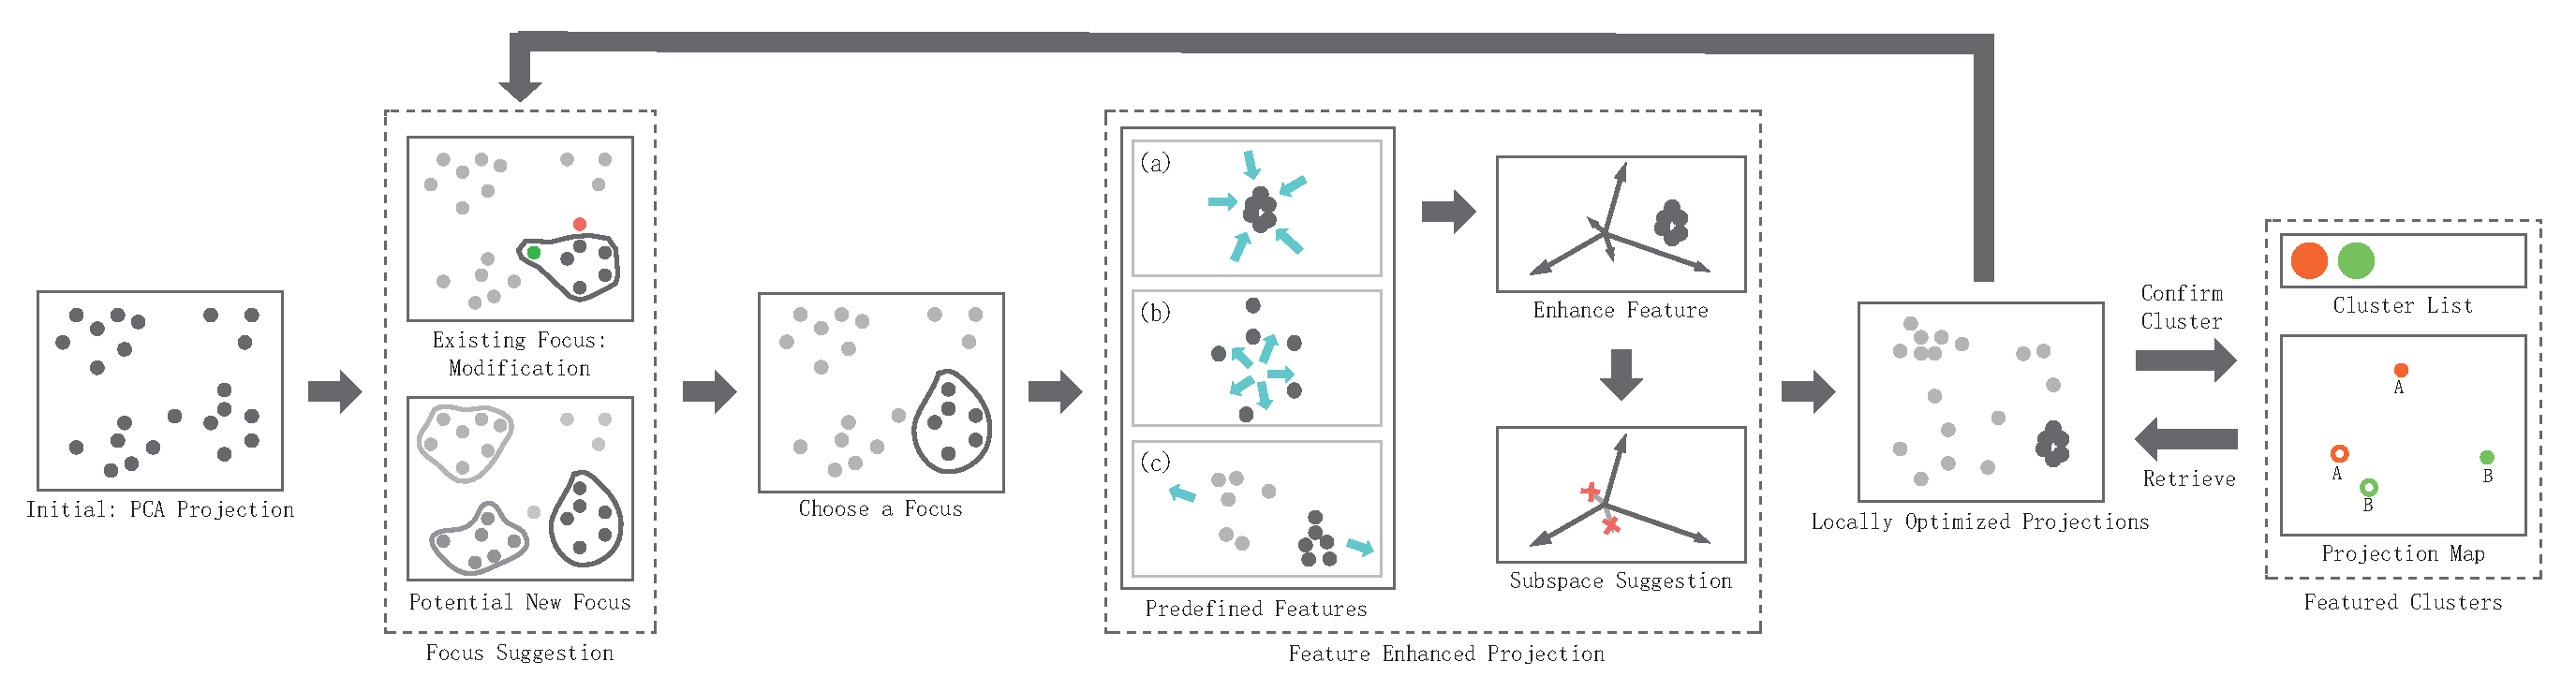
\includegraphics{images/Pipeline.eps}
\caption{Sample illustration.}
\end{figure*}
\else
\begin{figure*}[htbp]
\centering
  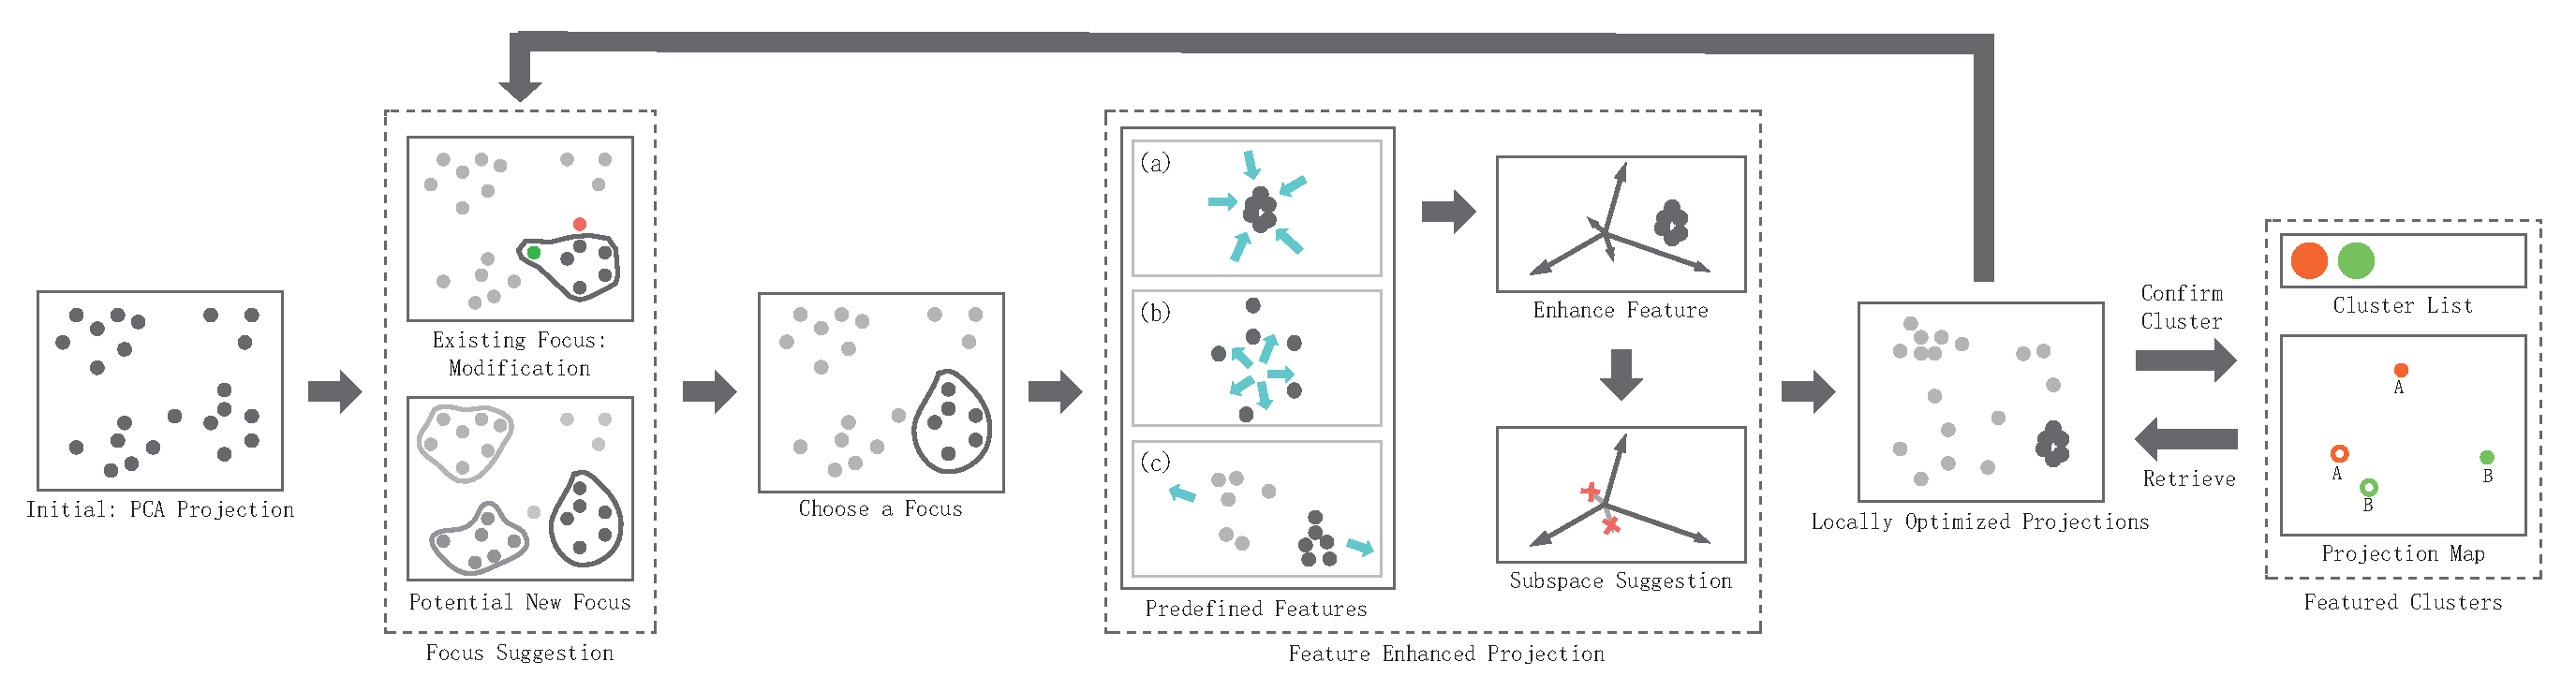
\includegraphics[width=1\linewidth]{images/Pipeline.eps}% 1\linewidth
  \caption{The overview of delivery system.}\label{fig.2}
  \end{figure*}
  \fi
\section{High-dimensional Local Data Analysis in Locally Optimized Projections}
As described in the workflow, the proposed method supports a four-step exploration. In this section, we'll elaborate details of our method in each step of the exploration process.
\label{section:method}
\subsection{Discovering Interesting Local Focus}
Following Shneiderman's suggestion~\cite{DBLP:conf/vl/Shneiderman96}, we first provide the PCA projection as an overview of the data. Then we help the user find an interesting subset as the focus of subsequent local analysis.

In a projection, there are two situations where some local data is considered interesting. The first case is about distance distortion. Incorrect distances result in false neighborhoods. Closely distributed data may be far away in the original space and vice versa. Data involved in a distorted local area is regarded informative in the projection. It's also the basic idea in previous works concerning about data locality~\cite{DBLP:journals/cg/MartinsCMT14}~\cite{DBLP:journals/tvcg/StahnkeDMT16}. But such analysis only focuses on each datum at a time. It's hard to describe a group of data in this context. That's why we consider the second type, where the data is involved in some featured relationships, like being an outlier or a cluster. The relationship may have been weakened (e.g. a false cluster), but it's still strong enough to appear in the current projection. Hence, it makes a reasonable focus for a further study. Besides, it's suitable to describe a group of data in the context of relationships, rather than distance errors.

To put it simply, distortion analysis focuses more on the neighborhood of a single datum. Relationship analysis promotes the study of a data group. Regarding the two cases, we adopt different means to help the user find an interesting local focus.

\subsubsection{Datum Suggestion Based on Distance Distortion}
For any given projection, we consider a datum interesting if its distances to other data have been severely distorted. To measure the distortion, we accumulate distance errors for each datum in the projection:
$$Error(\mathbf{x}_{i}^{\prime}) = \sum\limits_{j=1}^{n}(Dist(\mathbf{x}_{i}, \mathbf{x}_{j}) - Dist(\mathbf{x}_{i}^{\prime}, \mathbf{x}_{j}^{\prime}))^{2}, i = 1,2,\cdots n$$
Here the $\mathbf{x}_{i}$ and $\mathbf{x}_{i}^{\prime}$ represents the original data and the projected data respectively. Distance is measured by the Euclidean distance metric, taking into account all dimensions. We use point size to encode the accumulated distortion of each datum, as shown in Figure. \col{(Figure to be added.)}

On the other hand, we provide interactive hints to reveal the real distances. The approach is similar to that used in~\cite{DBLP:journals/tvcg/StahnkeDMT16}, but uses a different metaphor. When user hovers on the projection, we construct a so-called 'high-dimensional lantern' using interpolation. Assume that the hovered position corresponds to a two-dimensional datum $\mathbf{p}^{\prime}$, we interpolate its high-dimensional counterpart as follows:
$$\mathbf{p} = \sum\limits_{i=1}^{n}\mathbf{w}_{i}\cdot\mathbf{x}_{i} =  \sum\limits_{i=1}^{n}\frac{Dist(\mathbf{x}_{i}^{\prime}, \mathbf{p}^{\prime})^{-1}}{\sum\limits_{j=1}^{n}Dist(\mathbf{x}_{j}^{\prime}, \mathbf{p}^{\prime})^{-1}}\cdot\mathbf{x}_{i}$$
The interpolation weight $\mathbf{w}_{i}$ of data $\mathbf{x}_{i}$ depends on its distance to the hovered spot in the projection. Closer data get larger weights. When user hovers right on $\mathbf{x}_{i}^{\prime}$, $\mathbf{w}_{i}$ equals $1$ while all the other weights get $0$. The result equals to the original data: $\mathbf{p} = \mathbf{x}_{i}$.

By the interpolation, we aims to infer what kind of data is desired by the user. Then this desired point acts as a high-dimensional lantern, shedding lights on all the other data to indicate their distances. With the lighting metaphor, we encode distance information using the saturation tunnel in HSL color space:
$$Saturation(\mathbf{x}_{i}^{\prime}) = \max{\{(\alpha D_{i}^{2} + \beta D_{i} + \gamma)^{-1}, 1\}},$$
$$D_{i} = Dist(\mathbf{x}_{i}, \mathbf{p}), \quad i = 1,2,\cdots n$$
The data gets high saturation, if it's close to the interpolated point in the original space. The parameters $\alpha,\ \beta$ and $\gamma$ come from the inverse-square law of the lighting model. Empirical values are chosen to accommodate most datasets. When some datum has a large distance distortion, its lights will not be able to illuminate its neighbors in the projection. In contrast, some far away points will be highlighted as the real neighbors. Figure. demonstrates the actual effect. \col{(Figure to be added.)}

In summary, large data points are potentially interesting data with high distortion and inconsistent illumination. With the hints, user hovers around the projection like experiencing an adventure. He holds a lantern to explore unknown structures in the complex data space. Compared to~\cite{DBLP:journals/tvcg/StahnkeDMT16}, this method enables a more smooth and natural perception of distance information.

\subsubsection{Cluster Suggestion Based on Projected Relationships}
Automatic clustering algorithms play an important role in previous works~\cite{DBLP:conf/ieeevast/NamHMZI07}~\cite{DBLP:journals/cgf/LeeKCSP12}~\cite{DBLP:journals/cgf/LiuWTBP15}. Users are either given the clustering results, or assisted in toning parameters of the algorithm. However, it's not intuitive to drive the clustering by parameters, since the algorithm is often a black box to users. Besides, it's hard for users to understand causes and details about the clusters, let alone modifying them or discovering new ones.

In our method, we decide not to provide global clustering results. Instead, we suggest an interesting group of data by examining projection clusters. It is based on the fact that, no additional or prior knowledge should be assumed in a free exploration. Users choose their focuses based on what they perceive. We only reveal real structures of the chosen focus. Users can still take full control of the clustering process, after they get the local insights.

Lots of clustering algorithms can be applied to identify projection clusters~\cite{DBLP:conf/ieeevast/Kandogan12}. We adopt a variant of DBSCAN~\cite{zhou2012research} whose parameters are adaptive to the data. We choose DBSCAN because it can efficiently identify clusters in any shape. The self-adaptive parameters make it applicable to most datasets without the need of manual toning. Refer to Figure. for the effect of cluster suggestion. \col{(Figure. to be added.)} Users can choose a suggested cluster by simply clicking on it. To be clear, the suggestion only clarifies dominant relationships perceived by the user. It doesn't provide any extra information beyond the projection. If the user doesn't feel satisfied with the suggestion, he can choose his own focus by brushing the data.

\subsection{Featured Projections of the Focus}
We call a chosen datum the focus point, and call a chosen group the focus group. After some focus is chosen, we generate projections to either reduce its distortion, or enhance its local relationships.

\subsubsection{Distortion Reduced Projection}
For a focus point, we seek a projection to reduce its accumulated distance distortions. Let $\mathbf{P}$ be the focus point, we aim to solve the following optimization problem:
$$\min Error(\mathbf{P}) = \min_{\mathbf{A}}  \sum\limits_{i=1}^{n}(Dist(\mathbf{P}, \mathbf{x}_{i}) - Dist(\mathbf{PA}, \mathbf{x}_{i}^{\prime}))^{2}$$
Here the term $\mathbf{A}$ represents the projection matrix. The projected focus point is $\mathbf{P^{\prime}} = \mathbf{PA}$. It can be proved that (see the appendix), the problem is equivalent to the following form:
$$\max_{\mathbf{A}}  \sum\limits_{i=1}^{n}Dist(\mathbf{PA}, \mathbf{x}_{i}^{\prime})^{2}$$
Note that if we replace the focus point with the center of data, the optimization will directly lead to PCA projection. In other words, PCA reduces global distortion by reducing the distortion of the average datum. In turn, we can see the problem as a 'center-shifted' PCA. The shifted center has the lowest distance distortion (see Figure.). \col{(Figure to be added.)} As a result, the neighborhood around the focus is more accurate. Compared to the simple correction used in~\cite{DBLP:journals/tvcg/StahnkeDMT16}, our linear projection can help maintain a consistent mental model of the data shape.

\subsubsection{Featured Local Relationships}
For a focus group, we first examine what kind of relationships are of interest in the local analysis. Since relationships are defined based on distances, we can take a look at the distance matrix. Given a focus, the distance matrix of all data is divided into three parts (see Figure. ). \col{(Figure to be added.)} The first part describes distances between group members. The second part is about distances between the group and the other data. The last part describes distances among the other data. Since the last part has nothing to do with the focus, we simply ignore it. For the remaining parts, we consider the chosen data to be either 'similar' or 'dissimilar'.

By revealing the similarities among group members, we show users in which aspects the data are most similar. It helps to comprehend why these data gather into a cluster in the projection. Enhancing dissimilarities, on the other hand, tells about the major differences among group members. Moreover, if there are sub-clusters within the group, the differences among them will be more prominent. This can reveal hidden local relationships.  Similarities between the group and the others is not of interest, as far as we are concerned. In contrast, by enhancing the dissimilarities, we can show why this group is different from the others. The idea resembles that of Linear Discriminant Analysis (LDA), expect that we did not regard the other data as a same class. In summary, three types of relationships are found most informative in the local analysis. We call them intra-group similarity, intra-group dissimilarity and inter-group dissimilarity respectively.

\subsubsection{Relationship Enhanced Projections}
With the three types of relationships, we fist translate them in the context of data distances. Then we adopt projection pursuit to find linear projections for the enhancement.

Enhancing similarities or dissimilarities, equals to decreasing or enlarging data distances in the projection. For a focus group $G$, we enhance the intra-group similarities by:
$$\min \sum\limits_{\mathbf{x}_{i}^{\prime}, \mathbf{x}_{j}^{\prime} \in G} Dist(\mathbf{x}_{i}^{\prime}, \mathbf{x}_{j}^{\prime})^{2} = \min_{\mathbf{A}} \sum\limits_{\mathbf{x}_{i}, \mathbf{x}_{j} \in G} Dist(\mathbf{x}_{i}\mathbf{A}, \mathbf{x}_{j}\mathbf{A})^{2}$$
For simplicity, we call this optimization the \textbf{Compress} metric, since the focus group will be compressed in the resulting projection. Likewise, we enhance the dissimilarities by minimizing the same metric:
$$\max_{\mathbf{A}} \sum\limits_{\mathbf{x}_{i}, \mathbf{x}_{j} \in G} Dist(\mathbf{x}_{i}\mathbf{A}, \mathbf{x}_{j}\mathbf{A})^{2}$$
We call this the \textbf{Expand} metric, as the opposite of Compress. It actually leads to a local PCA projection. At last, we enhance the inter-focus dissimilarities by enlarging distances between the group and the other data:
$$\max_{\mathbf{A}} \sum\limits_{\mathbf{x}_{i} \in G} \sum\limits_{\mathbf{x}_{j} \in \bar{G}} Dist(\mathbf{x}_{i}\mathbf{A}, \mathbf{x}_{j}\mathbf{A})^{2}$$
This one is called the \textbf{Separate} metric. Figure. illustrate the three concepts. In fact, we can see the focus point as a group containing only one datum. There will not be Compress or Expand projections. But the Separate metric is exactly the same as point-based distortion reduction. It enables us to combine all featured projections into the same framework.

\subsubsection{Subspace Suggestion}
All dimensions are considered when pursuing the featured projections. However, only a few of them truly contribute to the features. The redundant dimensions will interfere with the analysis. That's why we need to reveal a subspace where features are most prominent.

In a sense, projection pursuit is a process to identify the most featured dimensions. We can make reliable suggestions according to its results. To be specific, we choose a subspace based on the projection found in the original space. Then in the chosen subspace, we do optimizations again to get the final results.

Given a projection, we first calculate the weight of each dimension:
$$W(d_{i}) = \left \|  \mathbf{a}_{i}\right \|_{2}, i = 1,2,\cdots m$$
Here, $\mathbf{a}_{i}$ is the projected unit vector of dimension $d_{i}$. Its squared length acts as the weight. Then we rank all dimensions according to their weights: $W(d_{1}^{*}) > W(d_{2}^{*}) > \cdots >W(d_{m}^{*})$. All weights sum to 1. We pick out those with large weights, until their sum exceeds a certain threshold:
\begin{equation*}
\begin{aligned}
&Subspace = \{d_{i}^{*}| i = 1,2, \cdots L \},\\
&s.t.\ \sum\limits_{j=1}^{L} W(d_{j}^{*}) \leq R \ \text{and}\ \sum\limits_{j=1}^{L+1} W(d_{j}^{*}) > R
\end{aligned}
\end{equation*}
The sum is called the \textbf{subspace score}. It indicates how strong the chosen subspace is related to the features. The threshold $R$ is 0.75 by default, cutting down at least $25\%$ redundant dimensions. Users are informed of the weights at any time. They can change $R$ to include or exclude dimensions. In the remaining subspace, we get the final result via a second-time projection pursuit. The refined projection will be easier to interpret with only the most featured dimensions. Nevertheless, users can always decide whether to accept the original results, or run an easierxtra subspace suggestion.

\subsection{Modifying the Focus}
For a focus point, a distortion reduced projection is the final step. But for a focus group, it still needs to be modified. The featured projections support this task, by revealing the local insights.

The Expand projection shows minor relationships hidden in the group. Sub-clusters and outliers can be found. It helps to trim the focus into a more consistent cluster. The Compress projection not only shows similar aspects within the group. There could be other data who resemble the focus in these aspects. They will be drawn closer to the group in the projection, claiming to be potential members. The user may have missed them when making the selection. This projection can be used to regain the missing parts. The Separate projection exhibits differences between the group and the other data. If there are boundary points, they will stand out in the projection. It facilitate the study of cluster boundaries. The above benefits largely owe to the combination of local optimization and focus + context technique. In previous works with only local projections~\cite{DBLP:journals/tvcg/YuanRWG13}, it's hard to modify a focus without any context information.

We support the modification by providing two other brushing modes. In the 'Increase' mode, whatever chosen by the user will be added into the focus group. In the 'Decrease' mode, the user can choose among group members without being affected by the other data. After the modification is made, all featured projections will be updated. Smooth transitions are applied during the update. We keep an orthogonal mapping in each frame of the transition~\cite{cook2004computational}, in order to help maintain an intact mental model of the data space. The user can continue the analysis and modification, until he gets a satisfying result.

\subsection{Focus Comparison in the Projection Map}
During the exploration, there will be times when the user needs to store the result. For example, when sub-clusters are found, the large cluster should be stored before the exploration goes into details. Besides, it's necessary to compare different focuses regarding their features. For these purpose, we provide the focus list, along with a map of all featured projections.

In the focus list, users can store the current focus or retrieve it at any time. Each focus is represented as a node (see Figure. ). Its size denotes the data size. Users can name a focus, or assign it some color. Specially, there is a fixed node called 'All Data'. Applying Expand metric to it will get the global PCA projection.

For every focus in the list, its featured projections are shown as glyphs in the projection map. Different glyphs represent different types of projections, as shown in Figure. \col{(Figure to be added.)} Dimension weights are also displayed to help compare the projections. Clicking on a glyph can retrieve the focus and the corresponding projection. To quantify distances between any two projection, we refer to the manifold learning domain. It has been proved that any two 2D projections lie on the same manifold, which is called the Grassmann manifold. We measure projection distances by geodesic distances on the manifold~\cite{absil2004riemannian}. The map is constructed based on the distance matrix, using Multidimensional Scaling (MDS).

In the projection map, users can compare features of different focuses. For example, two focus groups may have the same reasons for the grouping (i.e. intra-group similarities), while having different inner-group diversities (see Figure.). \col{(Figure to be added.)} It helps to understand different local data in the context of featured dimensions. In addition, users can plan their own high-dimensional tours in this map. A similar idea has been proposed in the TripAdvisor~\cite{DBLP:journals/tvcg/NamM13}, as an extension of the Grand Tour~\cite{asimov1985grand}~\cite{cook1995grand}. But their projections are driven by dimensions without explicit semantics. In comparison, each spot in our map is tightly related to some local data and a certain relationship. It makes the tour more targeted and easier to interpret.
\section{Case Study}
\label{section:casestudy}
In this section, we demonstrate the effectiveness of our method with two real-world datasets.

\subsection{Cars Data}
\label{case:car}
For the first case, we present a neighborhood study on the Cars dataset~\cite{Lichman:2013}. The dataset contains 392 cars with 8 attributes: displacement, MPG, cylinder number, horsepower, weight, acceleration time, year and origin.

\begin{figure}[htbp]
\centering
  \includegraphics[width=0.7\linewidth]{images/car_1.eps}% 1\linewidth
  \caption{Car Data: In the global projection~(a), we find a misplaced datum with the help of focus point suggestion~(b). The Separate projection reduces its distortions~(c). We choose a neighborhood here, return to the overview (d) and compare with (b) to validate the results. See Section~\ref{case:car} for more details.}
\label{fig:car}
  \end{figure}

Figure~\ref{fig:car}(a) shows a global projection of the data. We activate the focus point suggestion to see the distortions, and search for a possibly distorted neighborhood. Note that large point size denotes high distortion level. We hover on the projection, and find an area where data points are generally large (Figure~\ref{fig:car}(b)). Then we hover on one large point (indicated by the pointer) to see its lighting. The lights should be able to indicate its real neighbors. As a result, some of the closest points are not highlighted, including two very large points in the locality. In contrast, some far away points get affected. They may be the real neighbors of the hovered datum. Therefore, we assume this point has large distortions, and choose it to be the focus.

We apply the Separate projection to reduce distortions regarding the focus point. As shown in Figure~\ref{fig:car}(c), the focus point (indicated by an arrow) who used to sit among the others, has moved to the periphery. The new layout successfully separates the focus from the other data. Then we activate the suggestion again, and find the focus to be rather small. Its lighting, when seeing closely, becomes more consistent in the neighborhood. That means close points in this view are probably the real neighbors. Moreover, most of the neighbors are also small. It proves that the projection do reduce distortions, not only for the focus point, but for its neighbors.

In order to validate the result, we choose some neighbors in a certain radius around the focus. Then we store them in the list, and turn back to observe them in the global projection (Figure~\ref{fig:car}(d)). Comparing Figure~\ref{fig:car}(b) and~\ref{fig:car}(d), we see that the chosen neighbors were mostly affected with deeper colors, when the focus was hovered. It turns out the closest neighbors are scattered quite randomly. We even find three far way neighbors at the left boundary of the zoomed area. It's impossible to separate the real neighbors from the false ones, without the help of our visual suggestions and the distortion-reduced projection.

\subsection{USDA Food Data}
\label{case:food}
The second case comes from the USDA Food Composition Data Set (http://www.ars.usda.gov/).  The dataset describes nutrients of a collection of raw or processed foods. After preprocessing, the dataset contains 722 records and 18 dimensions. It has been used in some previous works~\cite{DBLP:conf/ieeevast/TatuMFBSSK12}~\cite{DBLP:journals/tvcg/YuanRWG13} for their case studies. However, their methods focus on subspace mining, while we concern more about analyzing a piece of local data.

As shown in the overview (Figure~\ref{fig:food1}(a)), there are roughly three projection clusters. We choose one as the focus, aiming to analyze what foods it may contain. We use the Expand projection to see its inner structures (Figure~\ref{fig:food1}(b)). There seem to be some patterns, but not so obvious. We seek for the subspace suggestion with the threshold $R$ being $0.75$. The threshold keeps unchanged in the following process. Within the suggested subspace, we can see a more clear separation between a large  cluster and some outliers (Figure~\ref{fig:food1}(c)). In fact, the outliers include two tiny clusters, dominating two dimensions (Vitamin D and Sodium) respectively. Turning back to the overview, we find that the outliers are scattered all over the local region (Figure~\ref{fig:food1}(f)). It's hard to recognize and remove them without a proper local projection. So far, it is the first-level local analysis.

Then we go into the large cluster, to study the second-level locality. The cluster is extracted from the focus using the Decrease mode. In the Compress projection (Figure~\ref{fig:food2}(c)), a three-dimensional subspace is suggested. It shows that cluster members generally contain much energy and water, but have lower carbohydrate than the others. No matter what foods they are, they are unlikely grains. The subspace gets a score of 0.88, implying that the feature is rather obvious. The Expand projection (Figure~\ref{fig:food2}(b)) has four suggested dimensions: Vitamin D, Vitamin B6, Vitamin A and Vitamin B12. The focus is divided into three smaller clusters, each dominating one or two dimensions.

The first cluster (Figure~\ref{fig:food2}(d)) scores high in Vitamin D and Vitamin B6. They are probably not vegetables and fruits, which are poor in Vitamin D. The Compress projection (Figure~\ref{fig:food2}(g)) degrades to a 2D plane without using subspace suggestion. It's a strong pattern that none of the members has any fiber or beta carotene. This confirms our previous guess. Hence, we come to a primary conclusion: this cluster are probably fishes or dairy products, which are rich in Vitamin D and Vitamin B6.

The second cluster (Figure~\ref{fig:food2}(e)) scores high in Vitamin A, which is a property of animal livers. But it's also relatively low in Vitamin D, B6 and B12. This is a feature of plant-based foods. Most unselected data (colored in gray) behave similarly. Since the featured projection (Figure~\ref{fig:food2}(h)) did not give further information, we simply assume the cluster to be vegetables or animal livers. Back in the overview (Figure~\ref{fig:food2}(j)), these data are very close to the unselected data, which coincides with the local observation.

The third cluster seems rich in Vitamin B12. We enhance its inner relationships, going down to a third-level analysis. Again, there is one big cluster with some outliers in the projection (Figure~\ref{fig:food3}(b)). We remove the outliers, and enhance similarities within the cluster. The Compress view (Figure~\ref{fig:food3}(d)) shows a strong pattern that no fiber or Vitamin C exists here. The subspace score reaches 0.99. We can safely conclude that these are animal-based foods. In the Expand projection (Figure~\ref{fig:food3}(c)), five dimensions are suggested. The data are very diverse along the axis of lipid, while they separate into two groups in the other four dimensions. They are possibly fishes or red meats. In the overview, the two clusters are very close, yet separable (Figure~\ref{fig:food3}(g), (h)).

\begin{figure}[htbp]
\centering
  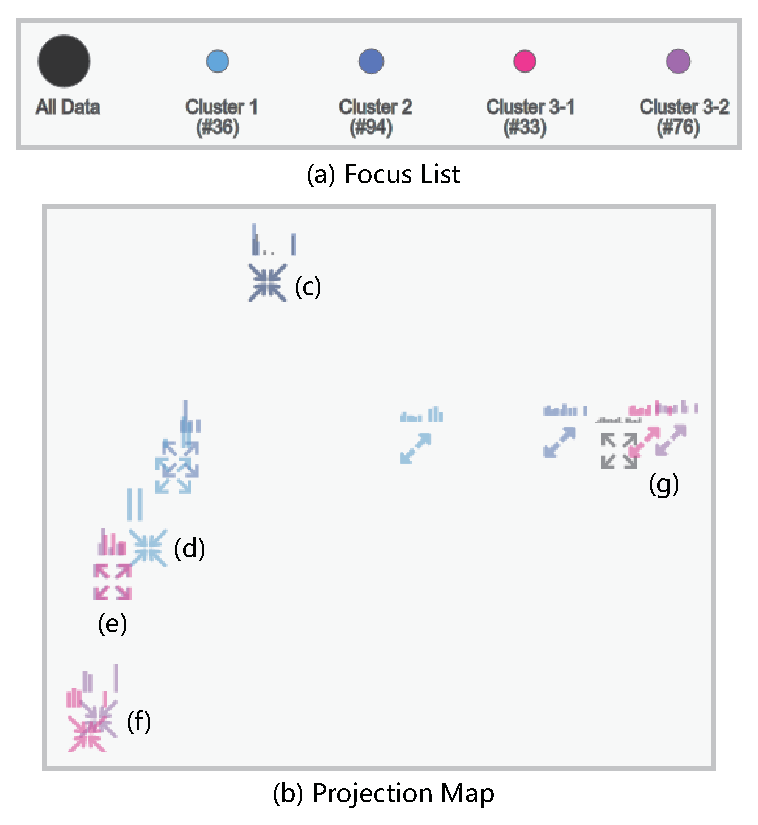
\includegraphics[width=0.85\linewidth]{images/map_1.eps}% 1\linewidth
  \caption{USDA Food Data: we choose a global cluster as the focus, and found outliers }
\label{fig:map}
  \end{figure}

In the above process, we have found outliers and hierarchical clusters in different levels of locality. The four clusters seem layered in the overview(Figure~\ref{fig:food2}(i), (j), Figure~\ref{fig:food3}(g), (h)). Without the featured local projections, it's hard for users to discover and interpret those clusters. Besides, the projections also help to understand the unselected data, and how the focus resembles or differs from them. This will be impossible if the context data are discarded in the projection.

\begin{figure*}[htbp]
\centering
  \includegraphics[width=0.97\linewidth]{images/food_1.eps}% 1\linewidth
  \caption{USDA Food Data: We choose a global cluster as the focus (a), and customize the projection to explore its features (b, c). Outliers can be found in the suggested subspace (d), which are hard to discern in the global projection (f). See Section~\ref{case:food} for more details.}
\label{fig:food1}
  \end{figure*}

\begin{figure*}[htbp]
\centering
  \includegraphics[width=0.97\linewidth]{images/food_2.eps}% 1\linewidth
  \caption{We focus on the cluster found in the subspace (Figure~\ref{fig:food1} (e)). Similarities (b) and diversities (c) are revealed among the cluster members. Three smaller clusters are found. One of them has a strong pattern that it contains no fibers of beta carotene (g). It could be a group of animal-based foods. See Section~\ref{case:food} for more details.}
\label{fig:food2}
  \end{figure*}

\begin{figure*}[htbp]
\centering
  \includegraphics[width=0.97\linewidth]{images/food_3.eps}% 1\linewidth
  \caption{We choose a sub-cluster found in Figure~\ref{food2}(f) to be the new focus. After removing some outliers within the cluster (b), we can see both strong features (d) and interesting inner structures (c) are revealed in the locally enhanced projections. Again, we find two sub-clusters (e, f) within the focus. They seem to be small neighboring clusters in the overview. See Section~\ref{case:food} for more details.}
\label{fig:food3}
  \end{figure*}

\note{compare to histograms: easy to find the most featured dimensions}
\section{Discussion}
\section{Conclusion}

%% if specified like this the section will be committed in review mode
\acknowledgments{
The authors wish to thank A, B, C. This work was supported in part by
a grant from XYZ.}

\bibliographystyle{abbrv}
%%use following if all content of bibtex file should be shown
%\nocite{*}
\bibliography{viewpointchanger}
\end{document}
